%The LHC and ATLAS are explained
%MC needs to be explained, how are systematics displayed
%DR and DS needs to be explained in the context of ATLAS


\chapter{The LHC and the ATLAS detector}
\label{lhc_atlas}


For most researches in modern particle physics there are two main constraints. The first one arises from the statistical nature of decay and creation processes in particle physics. Many of the most interesting events occur extremely rarely and call for large amount of data, more precisely high luminosity, to achieve significant results. Secondly the energy scale of particle physics is enormously high to allow breaking the structure of particles below the nuclear scale. 

This work was carried out using simulations based on the ATLAS~\cite{atlas} detector at the Large Hadron Collider (LHC)~\cite{lhc_machine} which offers both a record energy and luminosity. This chapter gives a summary of both machines and the knowledge necessary to understand the simulations used. First of a summary of the machines' parts and their technical details to are given, followed by a description of how the detector detects particles and how their properties are measured.

\section{Large Hadron Collider}

The Large Hadron Collider located at the facilities of the European Organization of Nuclear Research (CERN) close to Geneva was built to extend the frontiers of modern particle physics by delivering high luminosities and reaching unprecedented high energies thereby providing the data for multiple particle physics experiments.

The LHC is a circular particle detector with a circumference of \SI{26.7}{\kilo \metre} designed to  accelerate and collide two counter-rotating beams of protons. The protons are accelerated in bunches of up to \num{d11} protons at  energies up to \SI{7}{\tera \electronvolt} and a luminosity of \SI{d34}{\per\square\cm \per\s} achieving the record center-of-mass energy of up to \SI{14}{\tera \electronvolt}. The bunches are pre-accelerated by a number of accelerators before being inserted in the last, so called storage ring. An overview of the acceleration system is given in figure \ref{fig:accelerator_complex} and for more detailed information see the LHC design report. ~\cite{lhc_machine}. 
The four interaction points, at which the beams are brought to collision, inhabit the main experiments of the LHC. Two of them are general purpose detectors, namely ATLAS~\cite{atlas} and CMS~\cite{cms}, the third is the LHCb~\cite{lhcb} focusing on \Pbottom physics and lastly ALICE~\cite{alice} used for investigating heavy ion collisions.Figure \ref{fig:LHC} shows a sketch of the LHC's location and the positions of the four main experiments.

\begin{figure}[htbp]
\centering
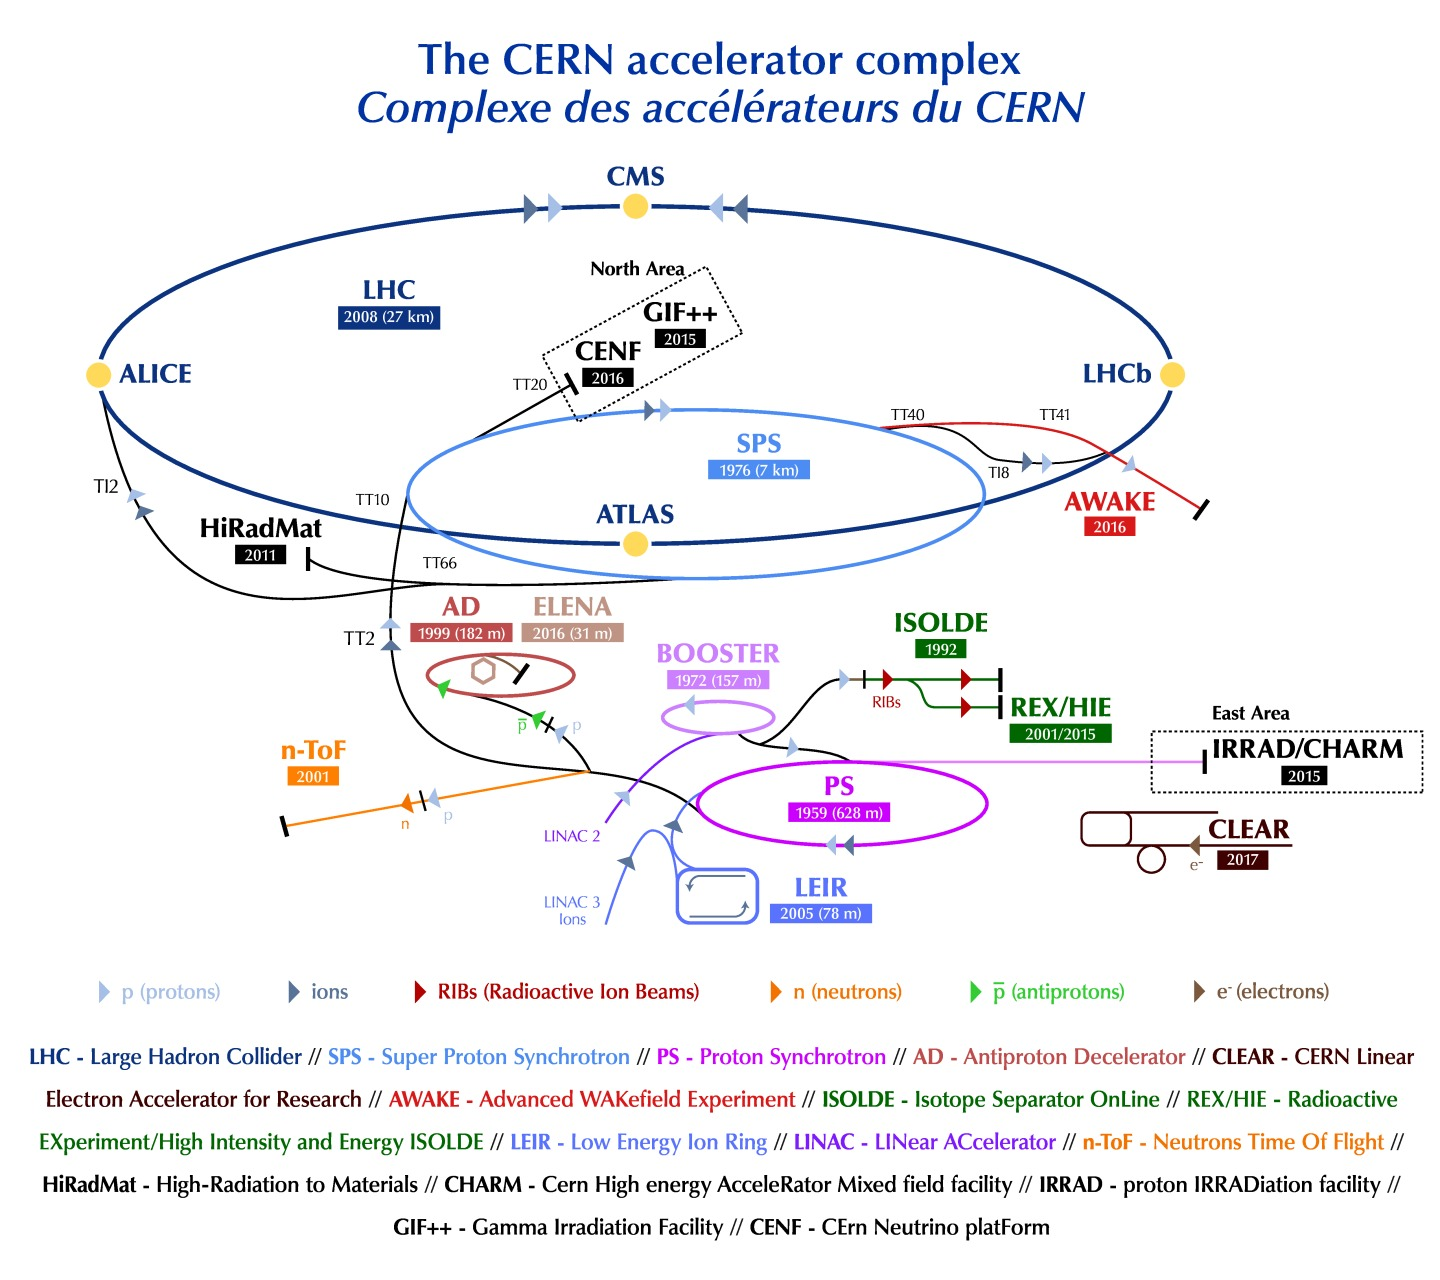
\includegraphics[width=\figwidth]{figures_LHC/CCC-v2018-print-v2.jpg}
\caption[Sketch of the LHC accelerator complex]{Sketch of the accelerator complex of the LHC showing the acceleration systems and the main storage ring with its experiments.~\cite{Mobs:2636343}}
\label{fig:accelerator_complex}
\end{figure}

\begin{figure}[htbp]
  \centering
  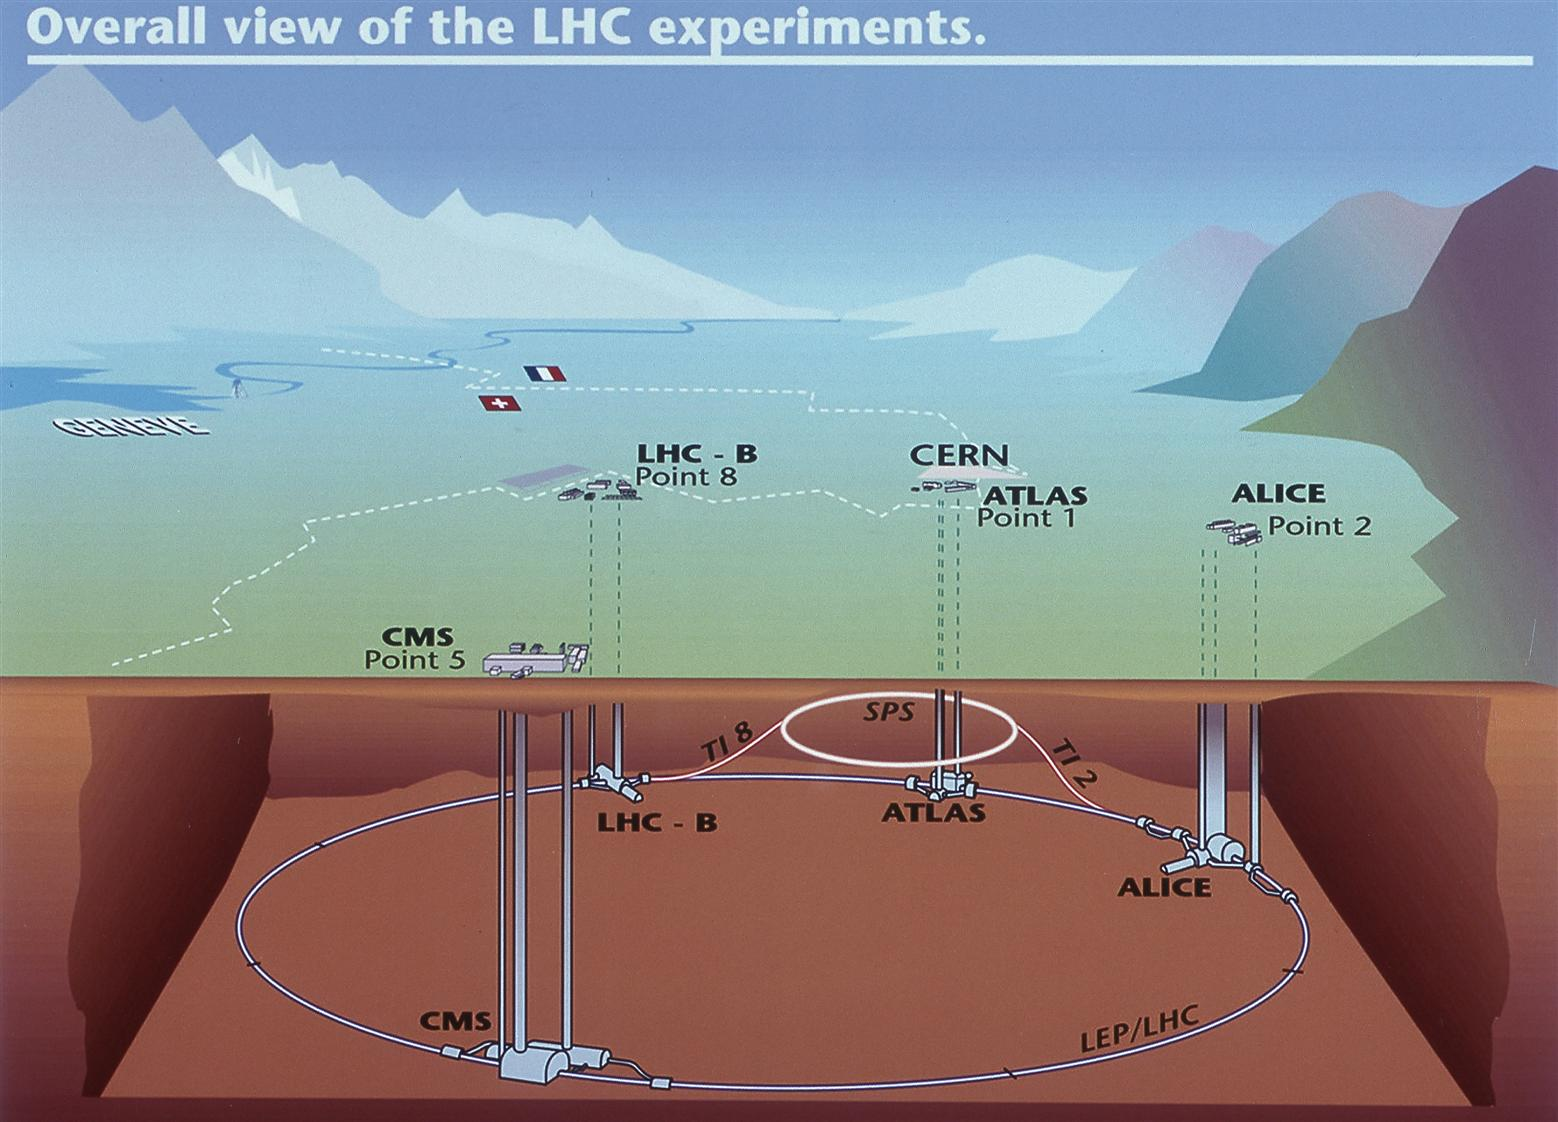
\includegraphics[scale=0.4]{figures_LHC/CERN-all-experiments.jpg}
  \caption[Sketch of the LHC ring.]{Sketch of the LHC ring, the position
    of the experiments and the surrounding countryside. The four big
    LHC experiments are indicated (ATLAS, CMS, LHC-B and ALICE) along with their injection lines (Point 1, 2, 4, 8).~\cite{Jean-Luc:841555}}
  \label{fig:LHC}
\end{figure}


\section{The ATLAS detector}

The ATLAS detector is a general purpose detector meaning it aims at covering a maximum number of final states, enabling reasearchers in may topics of particle physics to use its data.

ATLAS, "A Toroidal LHC Apparatus" has the distinguishing structure of a general purpose detector, its innermost part formed by tracking detectors directly surrounding the interaction point, followed by calorimeters and a further tracking detector for muon detection as the outermost component. All the components are visualized in figure~\ref{fig:atlas} including two humans to give an impression of the scale.

The innermost tracking detectors are summarized under the name Inner Detector (ID) and consist of two Silicon detectors namely the Pixel Detector and the Semi Conductor Tracker as well as a straw detector named Transition Radiation Tracker. The Inner Detector allows for precise measurement of not only charged particles' position and thus vertex information, but also for their charge and momentum.

The two calorimeters, being the electromagnetic calorimeter and the hadronic calorimeter, allow to measure the energy of particles by stopping them in the detector material.

The Muon Spectrometer is a further tracking detector identifying particles crossing it as muons, as all other charged particles are usually stopped in the other components.

In the following the concept of each detector component is briefly introduced~\cite{wermes} to then summarize how particles can be detected and distinguished.



\begin{figure}[htbp]
  \centering
  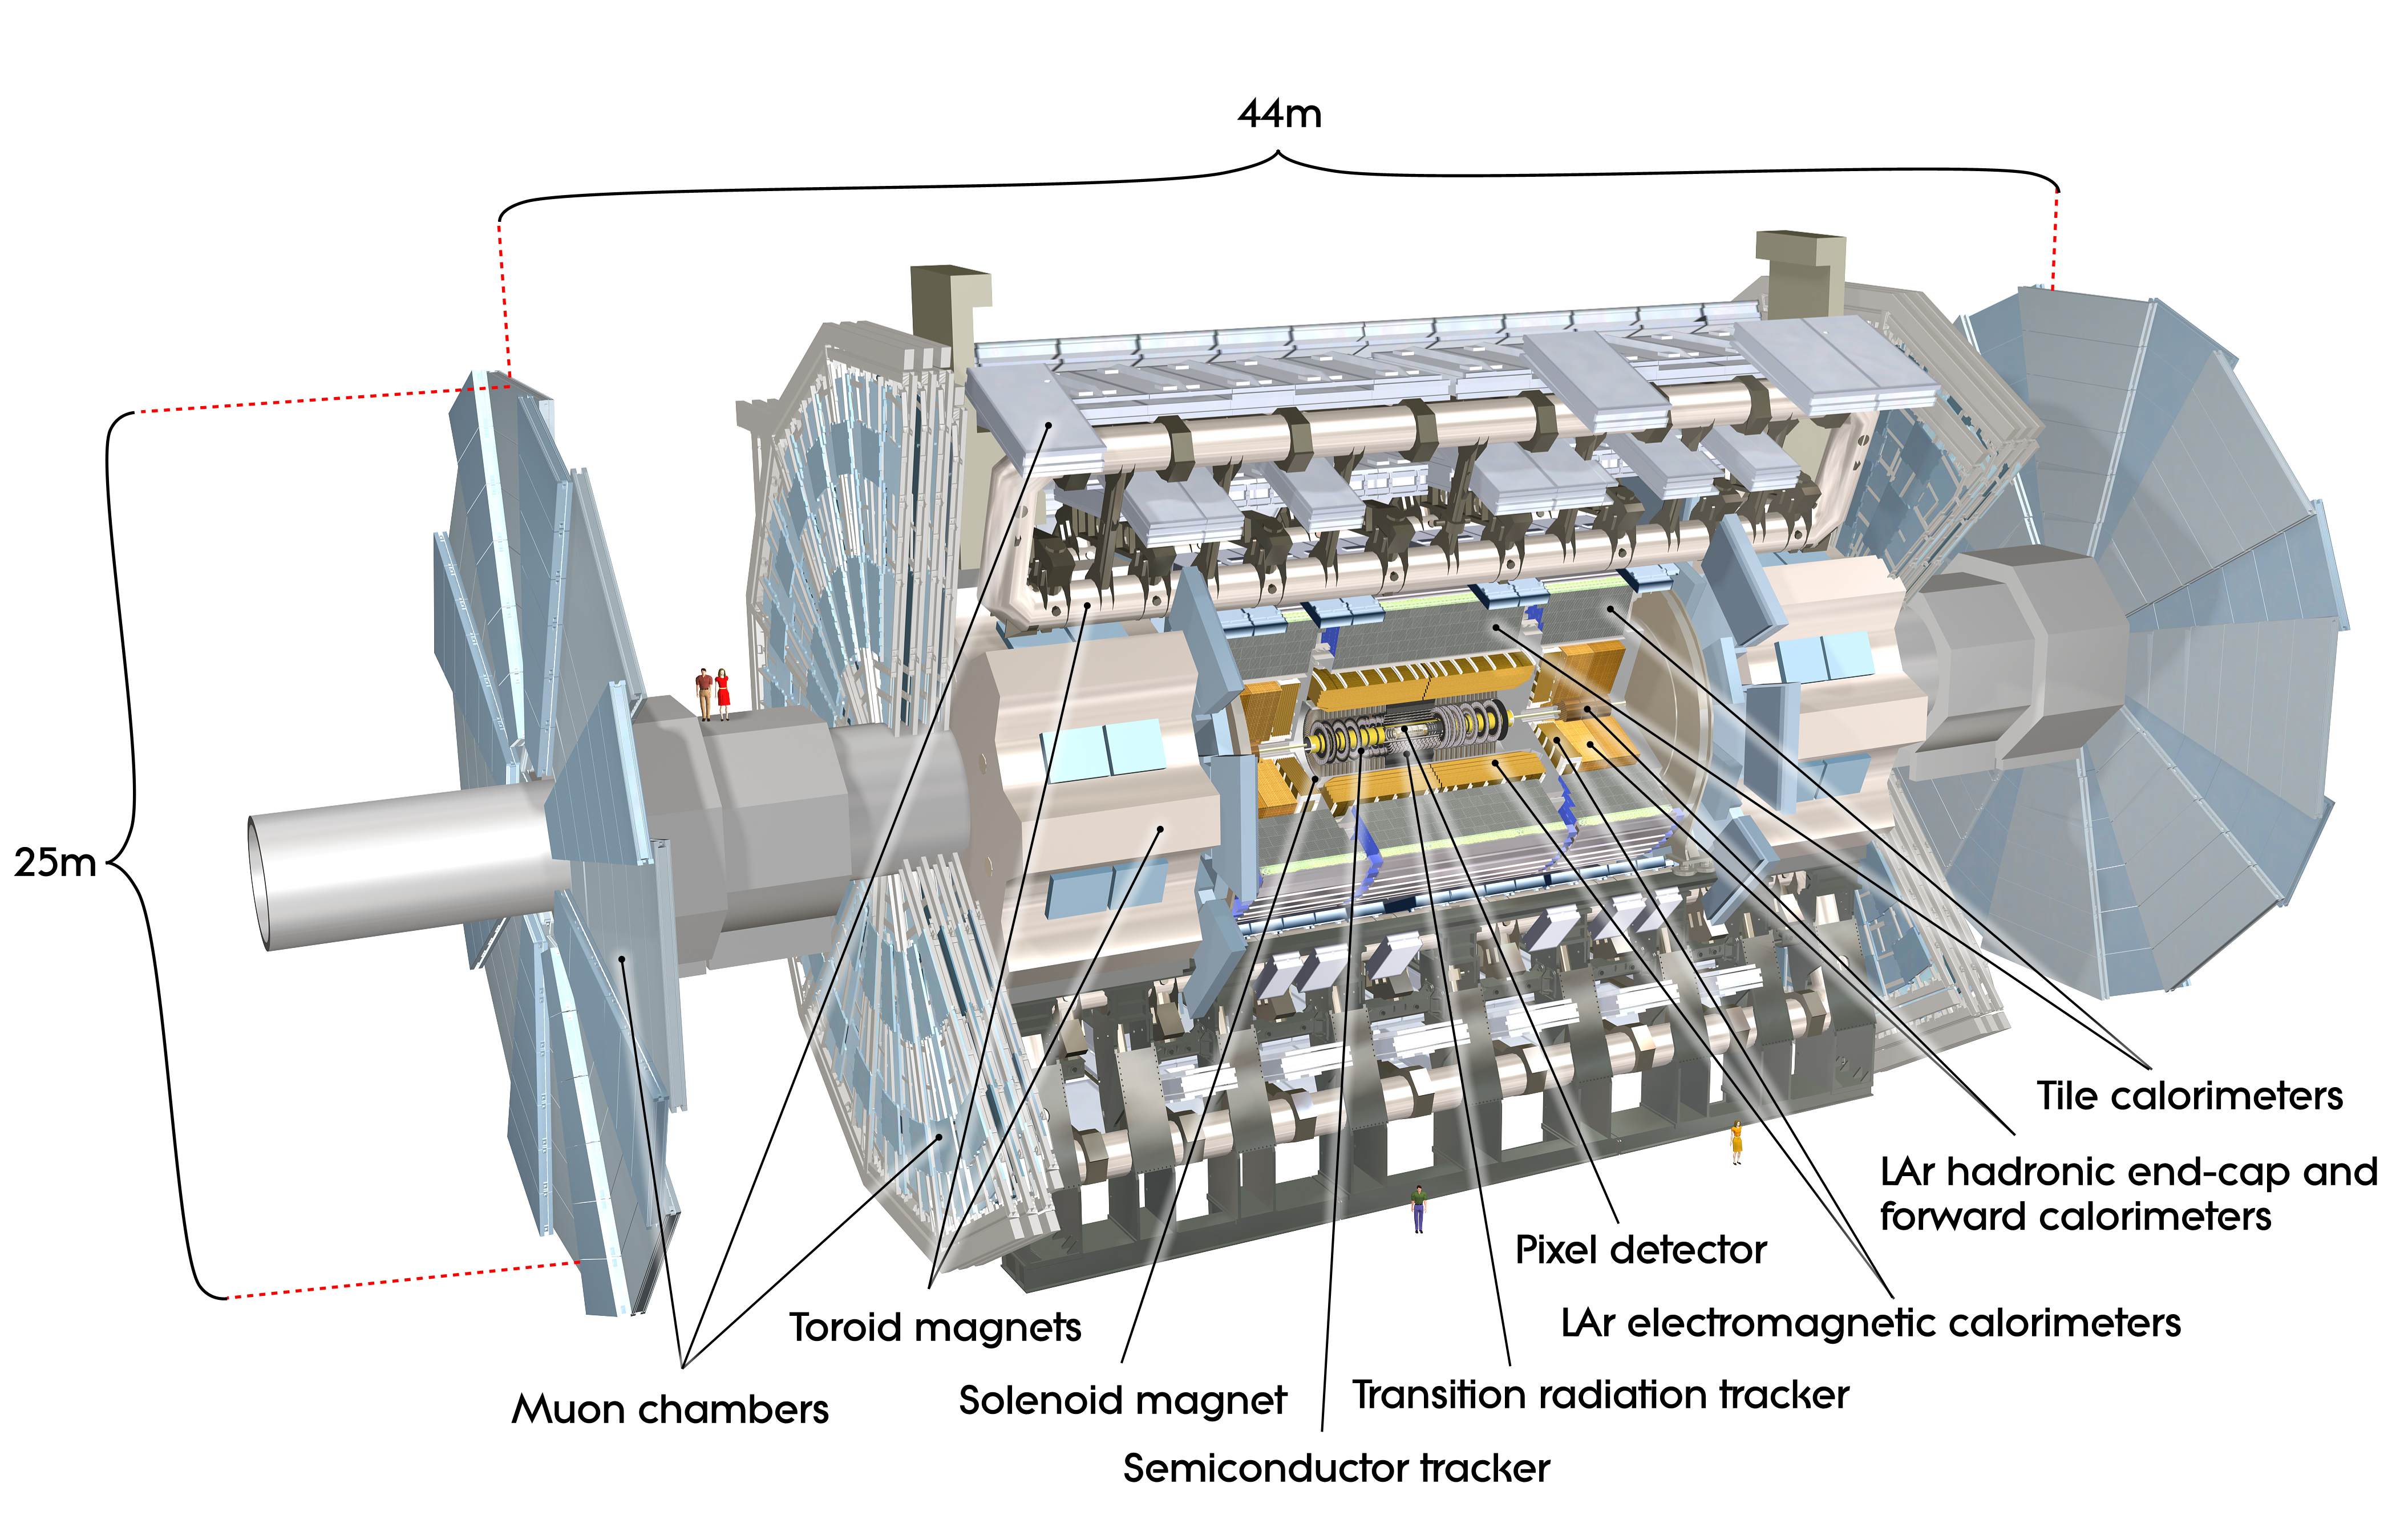
\includegraphics[scale=0.15]{figures_LHC/atlas-detector}
  \caption[Sketch of the ATLAS detector]{Sketch of the ATLAS detector and all its components including two average humans for scale.~\cite{Pequenao:1095924}}
  \label{fig:atlas}
\end{figure}


\subsection{Tracking detectors}

Tracking detectors are used to measure a charged particle's trajectory, momentum and charge value, of which two types are used in the ID of the ATLAS detector. The Pixel detector and the Semi Conductor Tracker (SCT) are silicon detectors and the Transition Radiation Tracker (TRT) is a straw-based tracking detector. For all detectors it holds true that they are surrounded by a magnetic field an cover a pseudorapidity range of $|\eta| < 2.5$. The magnetic field results in curved trajectories enabling an estimate of momentum and charge.\cite{leo}

Pixel detectors are based on ionisation of charged particles in the semiconductor material. The induced charged is picked up by the detector's pixels providing a position information. To provide a 3-dimensional trajectory the pixel-chips are ordered in 4 layers around the beam pipe where the layer closest to the point of interaction called Insertable B-Layer (IBL) was added in 2015. It is located only \SI{3.3}{\centi \metre} from the beam pipe and allows to detect vertices very close to the interaction point mainly originating from \Pbottom quarks giving the layer its name.~\cite{pixel_run2}

The SCT as a silicon microstrip detector is the second silicon-based tracker immediately following on the pixel detector. It consists of modules of four silicon strip sensors organised in four barrel layers and eighteen planar endcap disks.

The TRT is structured in straw tubes each tube being an individual drift chamber with a strong potential difference due to negatively charged walls. The tubes are filled by a gas mixture (xenon or argon) causing transversing charged particles to ionize and then by accelerated to the walls. A cascade is initiated and a measurable signal in the potential difference is measured. 
Between the tubes material is inserted resulting in transition radiation. This radiation has a cross section way higher for electrons thus adding particle information to the track information provided by the TRT.

A particle being detected in a layer of the ID is called a hit. The record of hits gives an estimate on the particle's trajectory and can thereby also give information on the vertex the particle originates from. This vertex information is worth mentioning as for a an experiment with an event count as large as the ATLAS experiment's events interfere and information from so called pileup events can affect the event's information. As pileup originates from different events it can be separated from the event of interest by separating the vertices.

\subsection{The ATLAS calorimeter system}

The ATLAS calorimter system is divided into three main parts. The electromagnetic (EM) calorimeter, compromising a barrel and two end-caps, and the hadron calorimter, built by a tile calorimeter, consisting of a a barrel and two so called "extended barrels", and the hadron end-caps. The third part is the forward calorimeter which additionally focuses on electromagnetic interaction. The tile calorimeter is scintillator-based apart from that the main part of the calorimeter system is based on liquid argon. The components cover a pseudorapidity range of $|\eta| < 4.9$

Calorimeters determine a transversing particle's energy by exploiting the formation of particle showers.~\cite{wermes} Due to inelastic collisions in the detector's material the energy of the original particle is distributed on a cascade of secondary particles finally stopped by ionization. The resulting charge or photons can be picked up as an estimate of the initial energy.

Electromagnetic calorimeters exploit the energy loss of electromagnetic interacting particles in matter. Mainly photons and electrons loose their energy based on pair production and Bremsstarhlung respectively. The energy loss initializes a cascade of particle decays called an electromagnetic shower.The decay stops when the shower particles do not hold sufficient energy for a decay anymore. The energy of the final state shower particles is picked up by the detector representing the initial particle's energy.
The ATLAS ECAL is a sampling calorimeter, built of two alternating layers of absorber and detection layer. In the absorber the showers are induced to then be detected in the detection layers.
shape, size, precision

As the ECAL uses electromagnetic showers the hadronic calorimeter depends on hadronic shower evolution. Hadronic showers are initialzed due to ionisation or strong interaction with the material's nuclei. If the resulting particles still interact with the material a shower evolves.

shape size precision

\subsection{The Muon spectrometer}

The second tracking detector of ATLAS is the muon spectrometer which is the outermost part of the detector. The task of the spectrometer is to detect charged particles transversing the calorimeter without being stopped or deploying their complete energy, and to do both collect trigger information and information on trajectory and momentum. Due to these two tasks the spectrometer is bifid with the first part being the trigger chamber covering a range of $|\eta|<2.4$, followed by the high-precision chamber with a range of $|\eta|<2.7$. The main detector's support feet cause a further gap at about $\phi = \ang{300}$ and $\phi = \ang{270}$.

Normally the only charged particles left to be detected in the muon spectrometer are muons giving the component its name and allowing to provide good trigger information for researches interested in muons in the final event topology.




\subsection{The ATLAS coordinate system}

The ATLAS coordinate system is a right-handed and right-angled coordinate system with the $z$-axis pointing along the LHC's beam pipe. The corresponding transverse plane is defined by the $x$-axis pointing towards the ring's centre while the $y$-axis points upwards. The origin of the system is defined by the nominal point of interaction. The polar angle $\theta$, is the angle between the $z$-axis and the $x$-$y$-plane and the azimuthal angle $\phi$ is the angle between the $x$- and the $y$-axis.

Alternatively, as in this work, an event's topology is described by the azimuthal angle $\phi$, the pseudo-rapidity $\eta$, and the transverse momentum $pT$. The pseudo-rapidity replaces the polar angle and is defined as

\begin{equation}
\eta = \frac{1}{2} ln\left[ tan\left(\frac{\theta}{2}\right)\right].
\end{equation}

The transverse momentum is defined by

\begin{equation}
pT = \sqrt{p_x^2 + p_y^2}
\end{equation}
where $p_x$ and $p_y$ are the momenta along the corresponding axes. 

The angular variables are defined within

\begin{equation}
\eta \in [-\infty,\infty],\,
\phi \in [-\pi,\pi].
\end{equation}

This cylindrical system makes use of the shape of the ATLAS detector and the momentum conversation of the transverse plane due to it being perpendicular to all initial beam momenta.

\subsection{Particle Detection in the ATLAS detector}

This section focuses on the detection and distinction of different particle types in the ATLAS detector. The capability and combined information of the detector components is introduced giving an explanation of the general working principle and also of the characteristics defining the events in this work. Figure \ref{fig:atlas_sketch} gives an overview of typical particle interactions and detections.

In order to reconstruct the particles in an event low level information is gathered using the direct detector output and then associated to the higher level particle information.

The information from the ID is called a track and contains not only the trajectory but also how consistently a track hs hits in every layer. A track offers momentum and charge information and can be associated with a vertex and a possible energy deposition in a calorimeter. 
The vertex reconstruction arising from the track information allows to define a primary vertex defined by the highest sum of squared transverse momenta while additional vertices are identified as pileup vertices.
Secondary vertices originating from tracks connected to the original vertex can be collected to identify short-lived particles.

The calorimeter data is summarised in clusters. Clusters are neighboring calorimeter cells with energy depositions significantly higher than the expected noise. A cluster is formed around a high energy deposition and can be associated to hadrons or jets or even to a corresponding track.



\begin{figure}[htbp]
  \centering
  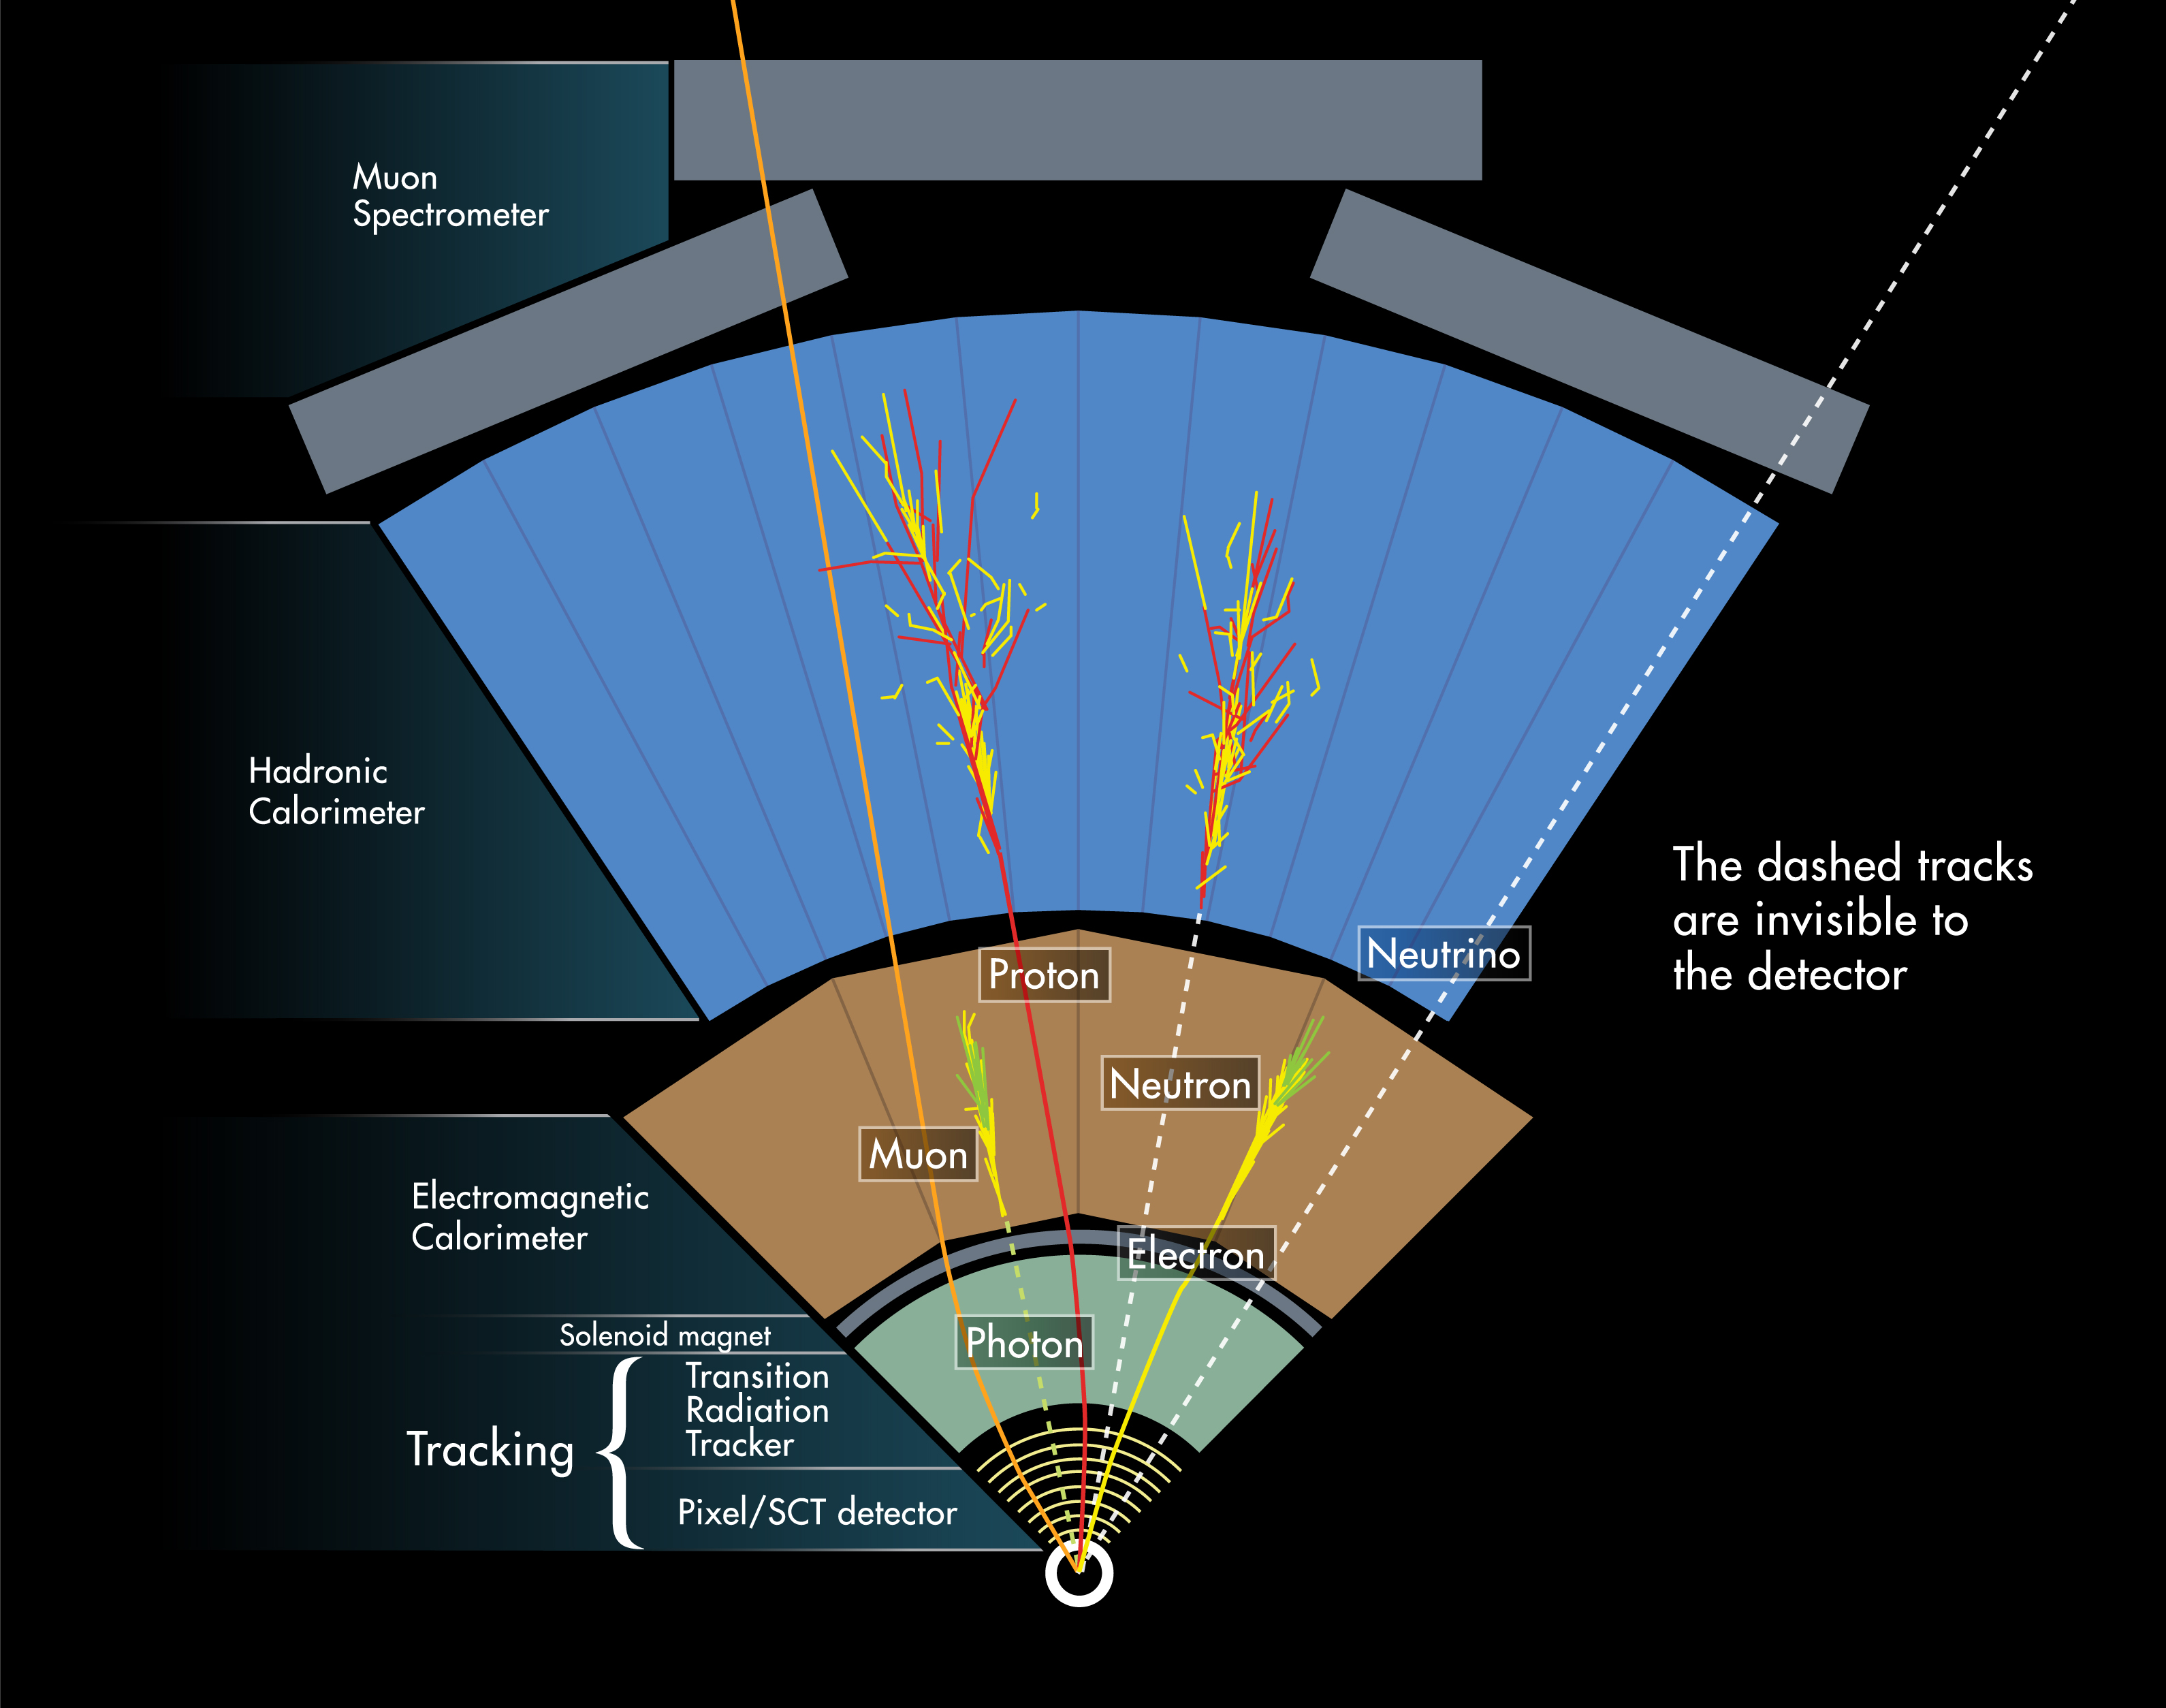
\includegraphics[scale=0.6]{figures_LHC/atlas-abstract}
  \caption[Scheme of the ATLAS-detector's detection procedure]{Scheme of the ATLAS-detector showing examples of tyical particle detections. \cite{Pequenao:1095924}}
  \label{fig:atlas_sketch}
\end{figure}

\section{Monte Carlo Simulation}

A Monte Carlo simulation is

detector simulation runs on top of Monte Carlo simulation

Simulations are based on cross sections which can be calculated and measured in units of \textsc{barn} where \SI{1}{\barn} = \SI{1e-28}{\square \metre}

Simulations heavily rely on quantities than can both be calculated and measured in an experiment thus allowing for predictions and also for  controlling the theoretical values.
In high energy particle physics there are mainly two such quantities cross section and branching ratio0

In collisions not only the valence quarks but also the sea quraks are relevant which can be explained by the valence quarks radiating gluons and quark antiquark pairs with no net flavour change.also explains the mass

\section{tW event topology}
